\iffalse
\documentclass[journal,11pt,onecolumn]{IEEEtran}
\usepackage{setspace}
\usepackage{gensymb}
\singlespacing
\usepackage[cmex10]{amsmath}
\usepackage{amsthm}
\usepackage{mathrsfs}
\usepackage{txfonts}
\usepackage{stfloats}
\usepackage{bm}
\usepackage{cite}
\usepackage{cases}
\usepackage{subfig}
\usepackage{longtable}
\usepackage{multirow}
\usepackage{enumitem}
\usepackage{mathtools}
\usepackage{tikz}
\usepackage{circuitikz}
\usepackage{verbatim}
\usepackage[breaklinks=true]{hyperref}
\usepackage{tkz-euclide} % loads  TikZ and tkz-base
\usepackage{listings}
\usepackage{color}    
\usepackage{array}    
\usepackage{longtable}
\usepackage{calc}     
\usepackage{multirow} 
\usepackage{hhline}   
\usepackage{ifthen}   
\usepackage{lscape}     
\usepackage{chngcntr}
\usepackage{float}
\DeclareMathOperator*{\Res}{Res}
\renewcommand\thesection{\arabic{section}}
\renewcommand\thesubsection{\thesection.\arabic{subsection}}
\renewcommand\thesubsubsection{\thesubsection.\arabic{subsubsection}}

\renewcommand\thesectiondis{\arabic{section}}
\renewcommand\thesubsectiondis{\thesectiondis.\arabic{subsection}}
\renewcommand\thesubsubsectiondis{\thesubsectiondis.\arabic{subsubsection}}
\renewcommand\thetable{\arabic{table}}
% correct bad hyphenation here
\hyphenation{op-tical net-works semi-conduc-tor}
\def\inputGnumericTable{}                                 %%

\lstset{
%language=C,
frame=single, 
breaklines=true,
columns=fullflexible
}
%\lstset{
%language=tex,
%frame=single, 
%breaklines=true
%}
\providecommand{\pr}[1]{\ensuremath{\Pr\left(#1\right)}}
\providecommand{\prt}[2]{\ensuremath{p_{#1}^{\left(#2\right)} }}        % own macro for this question
\providecommand{\qfunc}[1]{\ensuremath{Q\left(#1\right)}}
\providecommand{\sbrak}[1]{\ensuremath{{}\left[#1\right]}}
\providecommand{\lsbrak}[1]{\ensuremath{{}\left[#1\right.}}
\providecommand{\rsbrak}[1]{\ensuremath{{}\left.#1\right]}}
\providecommand{\brak}[1]{\ensuremath{\left(#1\right)}}
\providecommand{\lbrak}[1]{\ensuremath{\left(#1\right.}}
\providecommand{\rbrak}[1]{\ensuremath{\left.#1\right)}}
\providecommand{\cbrak}[1]{\ensuremath{\left\{#1\right\}}}
\providecommand{\lcbrak}[1]{\ensuremath{\left\{#1\right.}}
\providecommand{\rcbrak}[1]{\ensuremath{\left.#1\right\}}}
\newcommand{\sgn}{\mathop{\mathrm{sgn}}}
\providecommand{\abs}[1]{\left\vert#1\right\vert}
\providecommand{\res}[1]{\Res\displaylimits_{#1}} 
\providecommand{\norm}[1]{\left\lVert#1\right\rVert}
%\providecommand{\norm}[1]{\lVert#1\rVert}
\providecommand{\mtx}[1]{\mathbf{#1}}
\providecommand{\mean}[1]{E\left[ #1 \right]}
\providecommand{\cond}[2]{#1\middle|#2}
\providecommand{\fourier}{\overset{\mathcal{F}}{ \rightleftharpoons}}
%\providecommand{\hilbert}{\overset{\mathcal{H}}{ \rightleftharpoons}}
%\providecommand{\system}{\overset{\mathcal{H}}{ \longleftrightarrow}}
	%\newcommand{\solution}[2]{\textbf{Solution:}{#1}}
\newcommand{\solution}{\noindent \textbf{Solution: }}
\newcommand{\cosec}{\,\text{cosec}\,}
\providecommand{\dec}[2]{\ensuremath{\overset{#1}{\underset{#2}{\gtrless}}}}
\newcommand{\myvec}[1]{\ensuremath{\begin{pmatrix}#1\end{pmatrix}}}
\newcommand{\mydet}[1]{\ensuremath{\begin{vmatrix}#1\end{vmatrix}}}
\providecommand{\rank}{\text{rank}}
\providecommand{\pr}[1]{\ensuremath{\Pr\left(#1\right)}}
\providecommand{\qfunc}[1]{\ensuremath{Q\left(#1\right)}}
	\newcommand*{\permcomb}[4][0mu]{{{}^{#3}\mkern#1#2_{#4}}}
\newcommand*{\perm}[1][-3mu]{\permcomb[#1]{P}}
\newcommand*{\comb}[1][-1mu]{\permcomb[#1]{C}}
\providecommand{\qfunc}[1]{\ensuremath{Q\left(#1\right)}}
\providecommand{\gauss}[2]{\mathcal{N}\ensuremath{\left(#1,#2\right)}}
\providecommand{\diff}[2]{\ensuremath{\frac{d{#1}}{d{#2}}}}
\providecommand{\myceil}[1]{\left \lceil #1 \right \rceil }
\newcommand\figref{Fig.~\ref}
\newcommand\tabref{Table~\ref}
\newcommand{\sinc}{\,\text{sinc}\,}
\newcommand{\rect}{\,\text{rect}\,}
\title{Assignment}
\author{dushyant | EE22BTECH11031}
\begin{document}
\newtheorem{theorem}{Theorem}[section]
\newtheorem{problem}{Problem}
\newtheorem{proposition}{Proposition}[section]
\newtheorem{lemma}{Lemma}[section]
\newtheorem{corollary}[theorem]{Corollary}
\newtheorem{example}{Example}[section]
\newtheorem{definition}[problem]{Definition}
\newcommand{\BEQA}{\begin{eqnarray}}
\newcommand{\EEQA}{\end{eqnarray}}
\newcommand{\define}{\stackrel{\triangle}{=}}
\bibliographystyle{IEEEtran}
\providecommand{\mbf}{\mathbf}
\providecommand{\pr}[1]{\ensuremath{\Pr\left(#1\right)}}
\providecommand{\qfunc}[1]{\ensuremath{Q\left(#1\right)}}
\providecommand{\sbrak}[1]{\ensuremath{{}\left[#1\right]}}
\providecommand{\lsbrak}[1]{\ensuremath{{}\left[#1\right.}}
\providecommand{\rsbrak}[1]{\ensuremath{{}\left.#1\right]}}
\providecommand{\brak}[1]{\ensuremath{\left(#1\right)}}
\providecommand{\lbrak}[1]{\ensuremath{\left(#1\right.}}
\providecommand{\rbrak}[1]{\ensuremath{\left.#1\right)}}
\providecommand{\cbrak}[1]{\ensuremath{\left\{#1\right\}}}
\providecommand{\lcbrak}[1]{\ensuremath{\left\{#1\right.}}
\providecommand{\rcbrak}[1]{\ensuremath{\left.#1\right\}}}
\theoremstyle{remark}
\newtheorem{rem}{Remark}
\providecommand{\abs}[1]{\left\vert#1\right\vert}
\providecommand{\res}[1]{\Res\displaylimits_{#1}} 
\providecommand{\norm}[1]{\left\lVert#1\right\rVert}
\providecommand{\mtx}[1]{\mathbf{#1}}
\providecommand{\mean}[1]{E\left[ #1 \right]}
\providecommand{\fourier}{\overset{\mathcal{F}}{ \rightleftharpoons}}
\providecommand{\system}[1]{\overset{\mathcal{#1}}{ \longleftrightarrow}}
\providecommand{\dec}[2]{\ensuremath{\overset{#1}{\underset{#2}{\gtrless}}}}
\let\vec\mathbf
\def\putbox#1#2#3{\makebox[0in][l]{\makebox[#1][l]{}\raisebox{\baselineskip}[0in][0in]{\raisebox{#2}[0in][0in]{#3}}}}
     \def\rightbox#1{\makebox[0in][r]{#1}}
     \def\centbox#1{\makebox[0in]{#1}}
     \def\topbox#1{\raisebox{-\baselineskip}[0in][0in]{#1}}
     \def\midbox#1{\raisebox{-0.5\baselineskip}[0in][0in]{#1}}
\maketitle
\textbf{Question:}Consider the probability space $(\Omega, \mathcal{G}, P)$, where 
   $ \Omega = \{1, 2, 3, 4\}$, 
    $\mathcal{G} = \{\emptyset, \Omega, \{1\}, \{4\}, \{2, 3\}, \{1, 4\}, \{1, 2, 3\}, \{2, 3, 4\}\}$, 
    $P(\{1\}) = \frac{1}{4}$.
Let $X$ be the random variable defined on the above probability space as
   $ X(1) = 1$, 
    $X(2) = X(3) = 2$, 
    $X(4) = 3$.
If $P(X \leq 2) = \frac{3}{4}$, then find $P(\{1, 4\})$ (rounded off to two decimal places).\\\hfill (GATE ST 2023)\\
\fi
\solution
\begin{table}[ht]
\centering
\caption{Probablity space}
\label{tab:2023/ST/60_1}
\begin{tabular}{|c|c|c}
\hline
Probablity space &Value \\ \hline
$\Omega$ & $\{1, 2, 3, 4\}$\\\hline
$\mathcal{G}$ &$\{\emptyset, \Omega, \{1\}, \{4\}, \{2, 3\}, \{1, 4\}, \{1, 2, 3\}, \{2, 3, 4\}\}$\\\hline
$P(\{1\})$ &$\frac{1}{4}$\\\hline
$P(X \leq 2)$ & $\frac{3}{4}$\\\hline
\end{tabular}
\label{tab:gate/st/60-1}
\end{table}
\\
\begin{table}[ht]
\centering
\caption{Random variable}
    \label{tab:GATE/ST/60_2}
\begin{tabular}{|c|c|c}
\hline
$X\brak{\Omega}$ & $\Omega$\\\hline
$\{1\}$ & 1\\\hline
$\{2,3\}$ &2\\\hline
$\{4\}$ & 3\\\hline
\end{tabular}
\label{tab:gate/st/60}
\end{table}
\\
Pmf is defined as\\
\begin{align}
p_x\brak{k} &= \begin{cases}
P(\{1\}) & ,k=1\\
P(\{2,3\}) &, k=2\\
P(\{4\}) &, k=3\\
\end{cases}
\end{align}
Values of P(\{2,3\}), P(\{4\}) are unknown, so let p, q be their respective values
\begin{align}
p_X\brak{k} &= \begin{cases}
\frac{1}{4} & ,k=1\\
p &, k=2\\
q &, k=3\\
\end{cases}
\end{align}
\begin{align}
\Pr{(\{1, 4\})} = p_X(1) +p_X(3)
\end{align}
We know\\
\begin{align}
p_X(1) +  p + q  &= 1
\end{align}
We can express Pr($X \leq 2$)as:
\begin{align}
\Pr{(X \leq 2)} &= p_X(1) + p\\
\end{align}
We can expres above equations as:
\begin{align}
\myvec{1 & 1
        \\1 & 0}\myvec{p \\q} = \myvec{\frac{3}{4}\\ \frac{1}{2}}
\end{align}
\begin{align}
p &= \frac{1}{2}, q =\frac{1}{4}
\end{align}
Finally
\begin{align}
\Pr{(\{1, 4\})} &= P(\{1\}) +q\\
\Pr{(\{1, 4\})} &= \frac{1}{4} + \frac{1}{4}\\
\Pr{(\{1, 4\})} &= 0.5
\end{align}
\begin{figure}[h]
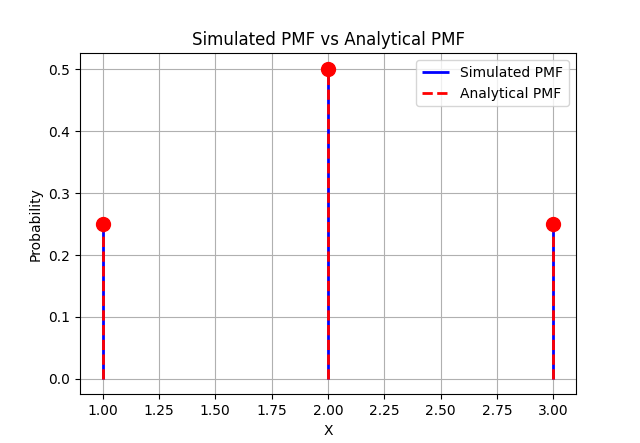
\includegraphics[width=\columnwidth]{figs/main2.png}
\caption{Analytical vs simulated}
\label{fig:GATE ST 60}
\end{figure}\\
Steps for simulating random variable.\\
\begin{enumerate}
\item Define the simulation size for datast (samples).
\item Assign calculated probablity for each probablity space p1, p2, p3, p4.
\item Define Random to generate a random number between 0 and 1.
\item Define the loop such that it generated number 1, 2, 3 for defined probablity space.
\item Store the simulated data in a .dat file.
\item Using matplotlib lib of python generate a V-line graph from the data in .dat file by counting the number of 1, 2, 3 .
\end{enumerate}

 
